% Выбор класса документа
\documentclass[14pt]{extarticle}
% Чтобы можно было использовать русские буквы в формулах ,
%но в случае использования предупреждать об этом
\usepackage{mathtext}
\usepackage{amsfonts}
\usepackage{layout}
\usepackage[height=25cm, a4paper, hmargin={3cm,1cm}]{geometry}

% Выбор внутренней TEX−кодировки
\usepackage[TS1,T2A]{fontenc}
\usepackage [utf8x] {inputenc}
\usepackage{amssymb}
\usepackage{amsmath, amsfonts, amssymb}
\usepackage{listings}
\usepackage{color}
\usepackage{graphicx}
\usepackage{multicol}
\usepackage{lipsum}
\usepackage{float}
\usepackage{adjustbox}
\usepackage{fancyhdr}
\usepackage{listings}
\usepackage{afterpage}
\usepackage{tikz}
\usetikzlibrary{patterns}
\usepackage{setspace}
\onehalfspacing
\usepackage[labelsep=period]{caption}
\lstset{
showspaces=false,
showtabs=false,
breaklines=true,
showstringspaces=false,
breakatwhitespace=true,
escapeinside={(*@}{@*)},
keywordstyle=\bfseries,
basicstyle=\ttfamily,
extendedchars=\true,
inputencoding=utf8x,
tabsize=2
}
\usepackage [english , russian] {babel}
\usepackage{etoolbox}
\addto\captionsrussian{\def\contentsname{Содержание}}
\addto\captionsrussian{\def\bibname{Список литературы}}
\renewcommand{\labelitemi}{---}
\renewcommand{\thesection}{\arabic{section}.}
\renewcommand{\thesubsection}{\arabic{section}.\arabic{subsection}.}
% Начинать первый параграф раздела следует с красной строки
\usepackage {indentfirst}
\parindent=1.25cm
% Конец преамбулы и начало текста
\begin{document}
%ТИТУЛЬНЫЙ ЛИСТ % % % % % % % % % % % % % % % % % % % % % % % % % % %
\thispagestyle{empty}
	\begin{center}
		\small
		МИНИСТЕРСТВО ОБРАЗОВАНИЯ И НАУКИ РОССИЙСКОЙ ФЕДЕРАЦИИ\\~ФГБОУ ВПО «СЫКТЫВКАРСКИЙ ГОСУДАРСТВЕННЫЙ УНИВЕРСИТЕТ ИМЕНИ ПИТИРИМА СОРОКИНА»\\
		ИНСТИТУТ ТОЧНЫХ НАУК И ИНФОРМАЦИОННЫХ ТЕХНОЛОГИЙ\\
		КАФЕДРА ПРИКЛАДНОЙ МАТЕМАТИКИ И ИНФОРМАЦИОННЫХ ТЕХНОЛОГИЙ В ОБРАЗОВАНИИ\\
	\end{center}
	\vspace{0.5cm}
	\begin{flushright}
		УТВЕРЖДАЮ\\
		Зав. кафедрой прикладной математики,\\
		к.ф.-м.н., доцент,\\
		\underline{\phantom{aaaaaaaaaaaa}}Ермоленко А. В.\\
		<<\underline{\phantom{aaaa}}>>\underline{\phantom{aaaaaaaaaaaa}} 2017г.\\
	\end{flushright}
	\begin{center}		
		\vspace{2.5cm}
		\large \textbf{ВЫПУСКНАЯ КВАЛИФИКАЦИОННАЯ РАБОТА}\\
		Тема: <<Генетические алгоритмы. Итеративный способ решения задачи раскроя>>
	\end{center}
	\begin{flushright}
		\small Научный руководитель\\к.ф.-м.н., доцент:\\\underline{\phantom{aaaaaaaaaaa}}А. А. Холопов\\
		<<\underline{\phantom{aaaa}}>>\underline{\phantom{aaaaaaaaaaa}} 2017г.\\
		\vspace{0.5cm}
		Исполнитель, студент\\145 группы:\\\underline{\phantom{aaaaaaaaaaa}}Мельников Вадим\\<<\underline{\phantom{aaaa}}>>\underline{\phantom{aaaaaaaaaaa}} 2017г.\\
	\end{flushright}
	\vspace{3cm}
	\begin{center}
		Сыктывкар 2017
	\end{center}
	\newpage
	%СОДРЕРЖАНИЕ % % % % % % % % % % % % % % % % % % % % % % % % % % % % % % % %
	\tableofcontents
	\thispagestyle{empty}
	\newpage
	\section{Введение в задачу раскроя материала}
	Экономия материала представляет собой сложную и важную проблему, с которой
	часто приходится встречаться на различных производствах, при резке различных материалов на: листы металла, стекла или дерева, трубы, профильный прокат, изделия сложной формы. Для её решения необходимо максимизировать использование материала, из которого вырезаются заготовки, что по сути и является рациональным раскроем материала. Максимизация использования материалов позволяет достичь большой экономии денежных средств.
	
	
	На самом деле, задача раскроя является NP-полной даже для прямоугольников. Для
	фигур неправильной формы геометрическая сложность увеличивает количество совершаемых вычислений, поэтому применяются различные эвристические методы решения задачи.
	\section{Основные характеристика задач раскроя}
	Прежде чем приступать к рассмотрению алгоритмов решения задачи раскроя, следует рассмотреть характеристики, влияющие на то, как будет выглядеть итоговый алгоритм решения. В статье \cite{Dyckhoff} Harald Dyckhoff приводит достаточно полное описание характеристик задач раскроя.
	\subsection{Пространственные характеристики}
	Основная характеристика раскроя --- количество измерений:
	\begin{itemize}
		\item раскрой в одномерном пространстве;
		\item раскрой в двумерном пространстве;
		\item раскрой в трёхмерном пространстве.
	\end{itemize}


	Например загрузка поддонов является задачей в двумерном пространстве. В отличие от 	задач в двух и более измерениях, задача в одномерном пространстве имеет явное решение. Достаточно подробно данная задача описывается в книге \cite{Cantorovich} Канторовича-Залгаллера --- <<Рациональный раскрой промышленных материалов>>. Так же в данной книге можно найти методы решения задач двумерного раскроя для случая прямоугольнных заготовок.
	\subsection{Количественные характеристики}
	Другая важная характеристика --- количественная. В задаче раскроя необходимо
	некоторым образом измерять количественные и качественные характеристики фигур.
	Например, площадь, длина и ширина фигур. Или количество уже расположенных фигур. Тут можно рассмотреть два варианта:
	\begin{itemize}
		\item дискретное измерение с помощью, например, натуральных и целых чисел;
		\item дробное измерение на основе вещественных чисел.
	\end{itemize}


	Первый вариант позволяет нам подсчитывать количество изделий, уже расположенных
	на материале, а с помощью второго можно измерять различные характеристики фигур, 	такие как площадь, длина и ширина.
	\subsection{Геометрические характеристики}
	Не малую роль играют в раскрое сами фигуры, которые необходимо расположить
	на плоскости. В пространстве фигуры однозначно определяются с помощью следующих
	свойств:
	\begin{itemize}
		\item формой;
		\item размером;
		\item ориентацией;
	\end{itemize}
	\subsection{Характеристики по ограничениям на результат}
	По ограничениям на результат можно выделить четыре основные группы:
	\begin{itemize}
		\item  минимальное расстояние между объектами;
		\item ориентация фигур относительно друг друга;
		\item ограничение на количество фигур;
		\item ограничение на количество совершаемых <<резов>>.
	\end{itemize}


	Автор \cite{Dyckhoff} выделяет ещё несколько групп по различным признакам, но данные являются
	основными.
	\section{Постановка задачи}
	Прежде чем переходить к алгоритмам, применяемым для решения задачи раскроя, следует рассмотреть постановку задачи. Задача в двумерном пространстве ставится по аналогии с задачей раскроя в одномерном пространстве \cite{Nikitenkov}, хотя одназначно с помощью математических соотношений описать её нельзя.
	
	Первоначально имеем множество фигур $F$ и $|F|=n$, плоскость с ширной $w$ и высотой $h$. Необходимо отыскать такое упорядоченное множество $F'$, что $F'\subset F$ и $|F'|\to \max$, при условии что все фигуры из $F'$ будут без пересечений размещены на плоскости с заданнами параметрами. 

	\section{Методы представления фигур для раскроя}
	Самым видимым атрибутом задач раскроя и тем, с чем сразу сталкиваются исследователи в данной области --- геометрическое представление фигур. Решение о том, 	как представлять фигуры, оказывает решающее значение на дальнейшую разработку системы.
	\subsection{Методы перемещения фигур}
	Прежде чем перейти к рассмотрению методов представления фигур, следует осветить важный вопрос, обычно опускаемый в литературе связанной с раскроем: <<Каким 	образом перемещать фигуры относительно друг друга?>>.


	Предположим, что мы уже некоторым образом расположили первую фигуру. Она распологается всегда в левом нижнем углу, как на рис. \ref{first_placed}. Для удобства, границы контейнера изображать не будем. Условимся, что вторая фигура в конечном расположении будет закрашена серым цветом.
		\begin{figure}[h]
		\begin{center}
			\begin{tikzpicture}
			\draw (0, 0)--(5, 0);
			\draw (5, 0)--(5, -1.25);
			\draw (5, -1.25)--(3.75, -1.25);
			\draw (3.75, -1.25)--(3.75, -2.5);
			\draw (3.75, -2.5)--(2.5, -2.5);
			\draw (2.5, -2.5)--(2.5, -1.25);
			\draw (2.5, -1.25)--(1.25, -1.25);
			\draw (1.25, -1.25)--(1.25, -2.5);
			\draw (1.25, -2.5)--(0, -2.5);
			\draw (0, -2.5)--(0,0);
			\end{tikzpicture}
		\end{center}
		\caption{Расположение первой фигуры}
		\label{first_placed}
	\end{figure}


	Самый первый метод, который будет интуитивно понятен всем --- <<лестничный>> или же	<<тетрисный>>. Его суть заключается в том, что мы двигаем фигуру вниз до первого столкновения с другой, потом также влево, потом опять вниз, и так далее пока фигура не перестанет смещаться. Рассмотрим на примере, как <<тетрисный>> способ расположит следующую фигуру. На рис. \ref{second_tetris} видно, что фигура перемещается слева направо с некоторым шагом по оси $x$ и в итоге находит углебление внутри другой фигуры.
	\begin{figure}[h]
		\begin{center}
			\begin{tikzpicture}
				\draw (0, 0)--(5, 0);
				\draw (5, 0)--(5, -1.25);
				\draw (5, -1.25)--(3.75, -1.25);
				\draw (3.75, -1.25)--(3.75, -2.5);
				\draw (3.75, -2.5)--(2.5, -2.5);
				\draw (2.5, -2.5)--(2.5, -1.25);
				\draw (2.5, -1.25)--(1.25, -1.25);
				\draw (1.25, -1.25)--(1.25, -2.5);
				\draw (1.25, -2.5)--(0, -2.5);
				\draw (0, -2.5)--(0,0);
				
				\draw (0.25, 1.5) circle (0.25);
				\draw (0.75, 1.5) circle (0.25);
				\draw (1.25, 1.5) circle (0.25);
				\draw (1.75, 1.5) circle (0.25);
				\draw (2.25, 1.5) circle (0.25);
				\draw (2.75, 1.5) circle (0.25);
				\draw (3.25, 1.5) circle (0.25);
				\draw (3.75, 1.5) circle (0.25);
				\draw (4.25, 1.5) circle (0.25);
				\draw (4.75, 1.5) circle (0.25);
				\draw (5.25, 1.5) circle (0.25);
				\draw (5.25, -2.25) circle (0.25);
				\draw (4, -2.25)[fill=gray!50] circle (0.25);
				
				\draw[->, thick] (0.25, 1.25) -- (0.25, 0);
				\draw[->, thick] (0.75, 1.25) -- (0.75, 0);
				\draw[->, thick] (1.25, 1.25) -- (1.25, 0);
				\draw[->, thick] (1.75, 1.25) -- (1.75, 0);
				\draw[->, thick] (2.25, 1.25) -- (2.25, 0);
				\draw[->, thick] (2.75, 1.25) -- (2.75, 0);
				\draw[->, thick] (3.25, 1.25) -- (3.25, 0);
				\draw[->, thick] (3.75, 1.25) -- (3.75, 0);
				\draw[->, thick] (4.25, 1.25) -- (4.25, 0);
				\draw[->, thick] (4.75, 1.25) -- (4.75, 0);
				\draw[->, thick] (5.25, 1.25) -- (5.25, -2);
				\draw[->, thick] (5, -2.25) -- (4.25, -2.25);
			\end{tikzpicture}
		\end{center}
		\caption{Расположение второй фигуры <<тетрисным>> способом}
		\label{second_tetris}
	\end{figure}


	Более сложный метод --- «метод сквозного прохода». Его основная идея заключается в том, что фигуру просто перемещают сквозь остальные и ищут подходящее ей место. Как 	видно на рис. \ref{second_through}, данный метод нашёл закрытую полость, до которой предыдущий способ дойти не смог.
	\begin{figure}[h]
		\begin{center}
			\begin{tikzpicture}
			\draw (0, 0)--(5, 0);
			\draw (5, 0)--(5, -1.25);
			\draw (5, -1.25)--(3.75, -1.25);
			\draw (3.75, -1.25)--(3.75, -2.5);
			\draw (3.75, -2.5)--(2.5, -2.5);
			\draw (2.5, -2.5)--(2.5, -1.25);
			\draw (2.5, -1.25)--(1.25, -1.25);
			\draw (1.25, -1.25)--(1.25, -2.5);
			\draw (1.25, -2.5)--(0, -2.5);
			\draw (0, -2.5)--(0,0);
				
			\draw (0.25, -2.25) circle (0.25);
			\draw[fill=gray!50] (1.5, -2.25) circle(0.25);
								
			\draw[->, thick] (0.5, -2.25) -- (1.25, -2.25);
			\end{tikzpicture}
		\end{center}
		\caption{Расположение второй фигуры способом <<сквозного прохода>>}
		\label{second_through}
	\end{figure}


	Самый сложный метод --- движение вдоль контура. Под контуром, в данном случае,
	подразумевается обновляемый контейнер. Изначально имеется некоторый контур пустого контейнера, затем в него добавляются одна за одной фигуры, и контур после расположения каждой из них изменяется. Таким образом, фигура движется вдоль контура контейнера, при нахождении подходящего места необходимо обновить контур с учетом расположения новой фигуры. На данный момент этот метод будет оставлен без особого внимания. Для его реализации необходимо создать цепь (растровую или же векторную) вдоль которой будет перемещаться фигура. Большую сложность, представляет в данном случае вопрос о выборе точки, относительно которой идёт движение.
	\subsection{Представление фигур в виде многоугольников}
	Представление фигур в виде многоугольников даёт хорошую точность аппроксимации. В таком представлении объем информации пропорционален числу вершин и не зависит от размера фигуры. Полигональное представление является первичным для фигур, а на его основе уже можно построить растровое представление, которое будет описано ниже.


	Полигональный метод хоть и даёт высокую точность представления, но имеет очень высокую вычислительную сложность --- $\mathrm{O}(e^n)$, где $n$ --- число вершин фигуры.


	Для того, чтобы проверить нет ли пересечений между какими-либо фигурами нужно
	выполнить следующий набор тестов \cite{Benell_Olivera}:
	\begin{enumerate}
		\item Проверить пересекаются ли описывающие прямоугольники фигур, если нет, то и фигуры не пересекаются, иначе перейти к следующему тесту.
		\item Для каждой пары рёбер проверить, пересекаются ли их описывающие прямоугольники.
		\item Проверить, пересекаются ли рёбра.
		\item Проверить, лежат ли какие-либо вершины одного полигона, внутри другого.
	\end{enumerate}
	\begin{figure}[h]
		\begin{center}
			\begin{tikzpicture}
				\draw (0.0, 0.0) -- (0.25, 2.0) -- (2.0, 1.8) -- (3.5, 2.5) --
								  (4, 0.5) -- (3.3, 1.1) -- (2.0, 1.1) -- (0, 0);
			
				\draw[fill=black] (0, 0) circle (0.075);
				\draw[fill=black] (0.25, 2.0) circle (0.075);
				\draw[fill=black] (2.0, 1.8) circle (0.075);
				\draw[fill=black] (3.5, 2.5) circle (0.075);
				\draw[fill=black] (4, 0.5) circle (0.075);
				\draw[fill=black] (3.3, 1.1) circle (0.075);
				\draw[fill=black] (2.0, 1.1) circle (0.075);
			\end{tikzpicture}
		\end{center}
		\caption{Представление фигуры при помощи многоугольника}
	\end{figure}


	Проверка на пересечения текущей фигуры с ранее расположенными может выполняться различными способами. Первый вариант --- через уравнение прямой с угловым коэффициентом. Этот метод для данной задачи будет излишним, ведь кроме проверки на пересечение двух отрезков, будут найдены точка пересечения и угловой коэффициент $k$ данной прямой. Также придётся проверять специальные случаи, когда прямые параллельны, когда они направлены вертикально вверх. Лучше использовать метод проверки на основе псевдоскалярного произведения, ведь тогда сильно снизится вычислительная нагрузка. Данный метод подробно рассматривается в задачах вычислительной геометрии \cite{Parsolov}.


	Для перемещения фигуры подходят только алгоритмы <<тетрисного>> движения. Применять «сквозное движение» мы не можем, так, как тогда придется постоянно проверять, не попала ли она внутрь другой, что в случае многоугольников сделать достаточно сложно. Для этого необходимо применять метод <<трассировки луча>> или приближённо считать комплексный интеграл, пользуясь интегральной формулой Коши \cite{Shabat}.


	Алгоритмы с представлением фигур в виде полигонов хорошо подходят для прямоугольников и несложных многоугольников с числом вершин до сотни. Для более сложных сильно возрастает время вычисления пересечений.


	Проблема данного метода состоит в сложности обработки контура. Построить эквидистантный (равноудалённый во всех точках от исходного) контур, чтобы задать зазор --- не
	такая уж лёгкая задача. Отделить внешний контур от внутренних тоже несколько сложнее,
	ведь контур может состоять из нескольких раздельных кривых, пусть и образующих в
	сумме одну замкнутую кривую.
	\subsection{Представление фигур в виде растровых матриц}
	Растровый метод, позволяет упростить геометрическую сложность фигуры и без дополнительных оптимизаций снизить сложность вычислений до $\mathrm{O}(n^2)$.


	Растровые методы предлагают разделить непрерывный раскройный лист на дискретные части, упрощая сложную геометрическую информацию до представления матрицей. Под матрицей будем понимать некоторое представление растра, в котором отмечены занятые и свободные места. Существуют различные методы представления.


	Самый простой метод представления --- это $1$ для занятого деталью места и $0$ для свободного. Раскраиваемый материал в данном случае представляется аналогично. На рис. \ref{first_rastr}
	можно увидеть первичный вариант растрового представления \cite{Benell_Olivera}. В данном случае занятые области отмечены серым цветом.

	Растровый способ не является первичным, он строится из фигуры, представленной многоугольником.
	Поэтому нельзя сразу говорить какие места заняты, а какие нет, ведь на входе имеется простое наложение многоугольника на растровую матрицу, что можно увидеть на рис. \ref{fig_on_rastr}.
	Рассмотрим возможный алгоритм закраски занятых областей:
	\begin{enumerate}
		\item На первом шаге имеется исходный многоугольник и пустой растр, как показано на рис. \ref{fig_on_rastr}. Выберем любое его ребро.
		\item Так как каждое ребро задается координатами $(x_1 , y_1 )$ и $(x_2 , y_2 )$, то на втором шаге можно получить уравнение прямой с угловым коэффициентом, которая содержит данный
		отрезок. Для определённости будем считать, что $y_1 \leq y_2$.
		\item Зададим множество $A=\{a_0, a_1, a_2, ..., a_{n-1}, a_n\}$, где $a_0=y_1$, а $a_n = y_2$. Остальные элементы являются целыми числами из интервала $(y_1, y_2)$.  
		\item Теперь, для каждой пары чисел $\{a_i, a_{i+1}\},\ i = 0:n-1$ из имеющегося уравнения прямой $y=kx+b$, вычислим $x_i$ и $x_{i+1}$.
		\item Вычислив, все необходимые координаты, можно отметить занятыми (на изображениях закрашены серым цветом), все клетки на отрезке заданном координатами $(x_i, a_i),\ (x_{i+1}, a_i)$.
	\end{enumerate}
	\begin{multicols}{1}
			\begin{figure}[H]
		\begin{center}
			\begin{tikzpicture}[box/.style={rectangle,draw=black, minimum size=0.5cm}]
			\foreach \x in {0,0.5,...,5}
			\foreach \y in {0,0.5,...,5}
			\node[box] at (\x,\y){};
			
			
			
			\foreach \x in {0, 0.5,...,5}
			\node[box, fill=gray] at (\x, 0){};
			
			\node[box, fill=gray] at (0, 0.5){};
			\node[box, fill=gray] at (0.5, 0.5){};
			\node[box, fill=gray] at (0.5, 1.0){};
			\node[box, fill=gray] at (0.5, 1.5){};
			\node[box, fill=gray] at (1.0, 1.5){};
			\node[box, fill=gray] at (1.0, 2.0){};
			\node[box, fill=gray] at (1.0, 2.5){};
			\node[box, fill=gray] at (1.0, 3.0){};
			\node[box, fill=gray] at (1.0, 3.5){};
			\node[box, fill=gray] at (1.5, 3.5){};
			\node[box, fill=gray] at (2.0, 3.5){};
			\node[box, fill=gray] at (2.0, 4.0){};
			\node[box, fill=gray] at (2.0, 4.5){};
			\node[box, fill=gray] at (2.5, 4.5){};
			\node[box, fill=gray] at (2.5, 5.0){};
			
			\node[box, fill=gray] at (5.0, 0.5){};
			\node[box, fill=gray] at (4.5, 0.5){};
			\node[box, fill=gray] at (4.5, 1.0){};
			\node[box, fill=gray] at (4.5, 1.5){};
			\node[box, fill=gray] at (4.0, 1.5){};
			\node[box, fill=gray] at (4.0, 2.0){};
			\node[box, fill=gray] at (4.0, 2.5){};
			\node[box, fill=gray] at (4.0, 3.0){};
			\node[box, fill=gray] at (4.0, 3.5){};
			\node[box, fill=gray] at (3.5, 3.5){};
			\node[box, fill=gray] at (3.0, 3.5){};
			\node[box, fill=gray] at (3.0, 4.0){};
			\node[box, fill=gray] at (3.0, 4.5){};
			
			\node[box, fill=gray] at (2.0, 2.0){};
			\node[box, fill=gray] at (2.0, 1.5){};
			\node[box, fill=gray] at (2.0, 1.0){};
			\node[box, fill=gray] at (2.5, 1.0){};
			\node[box, fill=gray] at (3.0, 1.0){};
			\node[box, fill=gray] at (3.0, 1.5){};
			\node[box, fill=gray] at (3.0, 2.0){};
			\node[box, fill=gray] at (2.5, 2.0){};
			
			
			\draw (0, 0) -- (5, 0);
			\draw (0, 0) -- (1.0, 2.1) -- (1.0, 3.1) -- (1.5, 3.6) -- (1.9, 3.6) -- (2.5, 5);
			\draw (5, 0) -- (4.0, 2.1) -- (4.0, 3.1) -- (3.5, 3.6) -- (2.9, 3.6) -- (2.5, 5);
			\draw (2.5, 1.5) circle (0.7);
			\end{tikzpicture}
		\end{center}
		\caption{Первичная растровая матрица}
		\label{first_rastr}
	\end{figure}
		\begin{figure}[H]
		\begin{center}
			\begin{tikzpicture}[box/.style={rectangle,draw=black, minimum size=0.5cm}]
				\foreach \x in {0,0.5,...,5}
					\foreach \y in {0,0.5,...,5}
						\node[box] at (\x,\y){};
			
				\draw (0, 0) -- (5, 0);
				\draw (0, 0) -- (1.0, 2.1) -- (1.0, 3.1) -- (1.5, 3.6) -- (1.9, 3.6) -- (2.5, 5);
				\draw (5, 0) -- (4.0, 2.1) -- (4.0, 3.1) -- (3.5, 3.6) -- (2.9, 3.6) -- (2.5, 5);
				\draw (2.5, 1.5) circle (0.7);
			\end{tikzpicture}
		\end{center}
		\caption{Наложение многоугольника на растровую матрицу}
		\label{fig_on_rastr}
	\end{figure}
	\end{multicols}

	Алгоритм рассматривает переход от отрезка к растру. Для перехода от многоугольника к растру достаточно повторить описанный алгоритм для всех его ребёр. В итоге получится то, что изображено на рис. \ref{first_rastr}.
	


	Операция проверки на пересечения с другими фигурами, при текущем расположении в координате $(x, y)$ фигуры с шириной равной $w$ и высотой $h$, не требует никаких сложных действий. Производится простое суммирование по следующей формуле:
	\begin{equation}
		\label{simple_sum}
		S = \sum_{i=1}^{h}\sum_{j=1}^{w}p_{i+y, j+x}f_{i,j} 
	\end{equation}


	В данном случае, $p_{i+y,j+x}$ --- значение в матрице раскройной плоскости со смещением на координату $(x, y)$, а $f_{i,j}$ --- значение в матрице фигуры. В случае если значение $S > 0$, то есть пересечение с некоторой фигурой, иначе его нет.


	Как видно на рис. \ref{first_rastr}, не все области внутри фигуры отмечены как занятые. В таком случае, некоторые фигуры могут попасть внутрь других, что будет являться ошибкой. Данная
	проблема может быть решена различными способами. Самый простой способ --- <<залить>> всё, что находится внутри внешнего конутура, отбрасывая пустоты внутри фигуры. Такой метод принесёт большие потери материала.


	Рассмотрим метод, позволяющий учитывать пустые места внутри фигур. Для начала необходимо отделить внешний контур фигуры:
	\begin{enumerate}
		\item Примем за текущую самую левую занятую точку с наименьшей ординатой.
		\item  Отметим текущую точку, как точку контура (на изображениях будет отмечаться диагональной штриховкой).
		\item Рассмотрим всех соседей текущей точки. Если есть соседняя точка, отмеченная цифрой $1$, переходим в данную точку и возвращаемся на второй шаг. Если текущая точка --- исходная, то закончить алгоритм, иначе повторить текущий шаг.
	\end{enumerate}


	Результат работы алгоритма можно увидеть на рис. \ref{result_contour}.
		\begin{figure}[H]
		\begin{center}
			\begin{tikzpicture}[box/.style={rectangle,draw=black, minimum size=0.5cm}]
			\foreach \x in {0,0.5,...,5}
				\foreach \y in {0,0.5,...,5}
					\node[box] at (\x,\y){};
				
			\foreach \x in {0, 0.5,...,5}
				\node[box, pattern=north west lines] at (\x, 0){};
				
			\node[box, pattern=north west lines] at (0, 0.5){};
			\node[box, pattern=north west lines] at (0.5, 0.5){};
			\node[box, pattern=north west lines] at (0.5, 1.0){};
			\node[box, pattern=north west lines] at (0.5, 1.5){};
			\node[box, pattern=north west lines] at (1.0, 1.5){};
			\node[box, pattern=north west lines] at (1.0, 2.0){};
			\node[box, pattern=north west lines] at (1.0, 2.5){};
			\node[box, pattern=north west lines] at (1.0, 3.0){};
			\node[box, pattern=north west lines] at (1.0, 3.5){};
			\node[box, pattern=north west lines] at (1.5, 3.5){};
			\node[box, pattern=north west lines] at (2.0, 3.5){};
			\node[box, pattern=north west lines] at (2.0, 4.0){};
			\node[box, pattern=north west lines] at (2.0, 4.5){};
			\node[box, pattern=north west lines] at (2.5, 4.5){};
			\node[box, pattern=north west lines] at (2.5, 5.0){};
			
			\node[box, pattern=north west lines] at (5.0, 0.5){};
			\node[box, pattern=north west lines] at (4.5, 0.5){};
			\node[box, pattern=north west lines] at (4.5, 1.0){};
			\node[box, pattern=north west lines] at (4.5, 1.5){};
			\node[box, pattern=north west lines] at (4.0, 1.5){};
			\node[box, pattern=north west lines] at (4.0, 2.0){};
			\node[box, pattern=north west lines] at (4.0, 2.5){};
			\node[box, pattern=north west lines] at (4.0, 3.0){};
			\node[box, pattern=north west lines] at (4.0, 3.5){};
			\node[box, pattern=north west lines] at (3.5, 3.5){};
			\node[box, pattern=north west lines] at (3.0, 3.5){};
			\node[box, pattern=north west lines] at (3.0, 4.0){};
			\node[box, pattern=north west lines] at (3.0, 4.5){};
			
			\node[box, fill=gray] at (2.0, 2.0){};
			\node[box, fill=gray] at (2.0, 1.5){};
			\node[box, fill=gray] at (2.0, 1.0){};
			\node[box, fill=gray] at (2.5, 1.0){};
			\node[box, fill=gray] at (3.0, 1.0){};
			\node[box, fill=gray] at (3.0, 1.5){};
			\node[box, fill=gray] at (3.0, 2.0){};
			\node[box, fill=gray] at (2.5, 2.0){};
			
			
			\draw (0, 0) -- (5, 0);
			\draw (0, 0) -- (1.0, 2.1) -- (1.0, 3.1) -- (1.5, 3.6) -- (1.9, 3.6) -- (2.5, 5);
			\draw (5, 0) -- (4.0, 2.1) -- (4.0, 3.1) -- (3.5, 3.6) -- (2.9, 3.6) -- (2.5, 5);
			\draw (2.5, 1.5) circle (0.7); 
			\end{tikzpicture}
		\end{center}
		\caption{Фигура с выделенным контуром}
		\label{result_contour}
	\end{figure}


	После отделения внешнего контура, необходимо отметить занятым, всё место между внешним контуром и контурами второго уровня. Это можно сделать следующим образом:
	\begin{enumerate}
		\item Первым шагом необходимо сохранить точки контура в отдельный массив и отметить их, как свободные (на изображениях не закрашены цветом) на растровой матрице.
		\item Далее, выполняется <<заливка>>. В процессе <<заливки>>, свободные клетки отмечаются как временно занятые (на изображениях будет изображаться перекрёстной штриховкой). Результат первых двух шагов приведён на рис. \ref{12fill_result}.
		\item\label{3fill_step} Третьим шагом инвертируем <<заливку>>. Для этого необходимо все временно занятые клетки надо отметить как своблдные. Свободные клетки необходимо отметить как временно занятые.
		Занятые клетки не затрагиваются. После этого можно вернуть на растровой матрице контур фигуры. Результат данного шага приведён на рис. \ref{3fill_result}.
		\item После этого опять выполняется <<заливка>>. Результат четвёртого шага приведён на рис. \ref{4fill_result};
		\item Последним шагом опять выполняется инверсия <<заливки>> по тем же правилам, что и на третьем шаге, только свободные клетки теперь отмечаются как занятые. Результат работы алгоритма приведён на рис. \ref{fill_result}.
	\end{enumerate}
	\begin{multicols}{1}
		\begin{figure}[H]
	\begin{center}
		\begin{tikzpicture}[box/.style={rectangle,draw=black, minimum size=0.5cm}]
			\foreach \x in {0,0.5,...,5}
				\foreach \y in {0,0.5,...,5}
					\node[box, pattern = crosshatch] at (\x,\y){};
					
				\node[box, fill=gray] at (2.0, 2.0){};
				\node[box, fill=gray] at (2.0, 1.5){};
				\node[box, fill=gray] at (2.0, 1.0){};
				\node[box, fill=gray] at (2.5, 1.0){};
				\node[box, fill=gray] at (3.0, 1.0){};
				\node[box, fill=gray] at (3.0, 1.5){};
				\node[box, fill=gray] at (3.0, 2.0){};
				\node[box, fill=gray] at (2.5, 2.0){};
				

				\node[box, fill=white] at (2.5, 1.5){};
				
			
		\end{tikzpicture}
	\end{center}
	\caption{Результат первых двух шагов алгоритма <<заливки>> пустых мест}
	\label{12fill_result}
\end{figure}
		\begin{figure}[h]
	\begin{center}
		\begin{tikzpicture}[box/.style={rectangle,draw=black, minimum size=0.5cm}]
			\foreach \x in {0,0.5,...,5}
				\foreach \y in {0,0.5,...,5}
					\node[box] at (\x,\y){};
					
				\node[box, fill=gray] at (2.0, 2.0){};
				\node[box, fill=gray] at (2.0, 1.5){};
				\node[box, fill=gray] at (2.0, 1.0){};
				\node[box, fill=gray] at (2.5, 1.0){};
				\node[box, fill=gray] at (3.0, 1.0){};
				\node[box, fill=gray] at (3.0, 1.5){};
				\node[box, fill=gray] at (3.0, 2.0){};
				\node[box, fill=gray] at (2.5, 2.0){};
				

				\node[box, pattern=crosshatch] at (2.5, 1.5){};
				
				\foreach \x in {0, 0.5,...,5}
					\node[box, pattern=north west lines] at (\x, 0){};
				
				\node[box, pattern=north west lines] at (0, 0.5){};
				\node[box, pattern=north west lines] at (0.5, 0.5){};
				\node[box, pattern=north west lines] at (0.5, 1.0){};
				\node[box, pattern=north west lines] at (0.5, 1.5){};
				\node[box, pattern=north west lines] at (1.0, 1.5){};
				\node[box, pattern=north west lines] at (1.0, 2.0){};
				\node[box, pattern=north west lines] at (1.0, 2.5){};
				\node[box, pattern=north west lines] at (1.0, 3.0){};
				\node[box, pattern=north west lines] at (1.0, 3.5){};
				\node[box, pattern=north west lines] at (1.5, 3.5){};
				\node[box, pattern=north west lines] at (2.0, 3.5){};
				\node[box, pattern=north west lines] at (2.0, 4.0){};
				\node[box, pattern=north west lines] at (2.0, 4.5){};
				\node[box, pattern=north west lines] at (2.5, 4.5){};
				\node[box, pattern=north west lines] at (2.5, 5.0){};
				
				\node[box, pattern=north west lines] at (5.0, 0.5){};
				\node[box, pattern=north west lines] at (4.5, 0.5){};
				\node[box, pattern=north west lines] at (4.5, 1.0){};
				\node[box, pattern=north west lines] at (4.5, 1.5){};
				\node[box, pattern=north west lines] at (4.0, 1.5){};
				\node[box, pattern=north west lines] at (4.0, 2.0){};
				\node[box, pattern=north west lines] at (4.0, 2.5){};
				\node[box, pattern=north west lines] at (4.0, 3.0){};
				\node[box, pattern=north west lines] at (4.0, 3.5){};
				\node[box, pattern=north west lines] at (3.5, 3.5){};
				\node[box, pattern=north west lines] at (3.0, 3.5){};
				\node[box, pattern=north west lines] at (3.0, 4.0){};
				\node[box, pattern=north west lines] at (3.0, 4.5){};
				
			
		\end{tikzpicture}
	\end{center}
	\caption{Результат третьего шага алгоритма <<заливки>> пустых мест}
	\label{3fill_result}
\end{figure}
	\end{multicols}
	\begin{multicols}{1}
		\begin{figure}[h]
	\begin{center}
		\begin{tikzpicture}[box/.style={rectangle,draw=black, minimum size=0.5cm}]
			\foreach \x in {0,0.5,...,5}
				\foreach \y in {0,0.5,...,5}
					\node[box] at (\x,\y){};
					
				\node[box, fill=gray] at (2.0, 2.0){};
				\node[box, fill=gray] at (2.0, 1.5){};
				\node[box, fill=gray] at (2.0, 1.0){};
				\node[box, fill=gray] at (2.5, 1.0){};
				\node[box, fill=gray] at (3.0, 1.0){};
				\node[box, fill=gray] at (3.0, 1.5){};
				\node[box, fill=gray] at (3.0, 2.0){};
				\node[box, fill=gray] at (2.5, 2.0){};
				

				\node[box, pattern=crosshatch] at (2.5, 1.5){};
				
				\foreach \x in {0, 0.5,...,5}
					\node[box, pattern=north west lines] at (\x, 0){};
				
				\node[box, pattern=north west lines] at (0, 0.5){};
				\node[box, pattern=north west lines] at (0.5, 0.5){};
				\node[box, pattern=north west lines] at (0.5, 1.0){};
				\node[box, pattern=north west lines] at (0.5, 1.5){};
				\node[box, pattern=north west lines] at (1.0, 1.5){};
				\node[box, pattern=north west lines] at (1.0, 2.0){};
				\node[box, pattern=north west lines] at (1.0, 2.5){};
				\node[box, pattern=north west lines] at (1.0, 3.0){};
				\node[box, pattern=north west lines] at (1.0, 3.5){};
				\node[box, pattern=north west lines] at (1.5, 3.5){};
				\node[box, pattern=north west lines] at (2.0, 3.5){};
				\node[box, pattern=north west lines] at (2.0, 4.0){};
				\node[box, pattern=north west lines] at (2.0, 4.5){};
				\node[box, pattern=north west lines] at (2.5, 4.5){};
				\node[box, pattern=north west lines] at (2.5, 5.0){};
				
				\node[box, pattern=north west lines] at (5.0, 0.5){};
				\node[box, pattern=north west lines] at (4.5, 0.5){};
				\node[box, pattern=north west lines] at (4.5, 1.0){};
				\node[box, pattern=north west lines] at (4.5, 1.5){};
				\node[box, pattern=north west lines] at (4.0, 1.5){};
				\node[box, pattern=north west lines] at (4.0, 2.0){};
				\node[box, pattern=north west lines] at (4.0, 2.5){};
				\node[box, pattern=north west lines] at (4.0, 3.0){};
				\node[box, pattern=north west lines] at (4.0, 3.5){};
				\node[box, pattern=north west lines] at (3.5, 3.5){};
				\node[box, pattern=north west lines] at (3.0, 3.5){};
				\node[box, pattern=north west lines] at (3.0, 4.0){};
				\node[box, pattern=north west lines] at (3.0, 4.5){};
				
				\foreach \y in {1, 1.5, ..., 5}
					\node[box, pattern=crosshatch] at(0, \y){};
				\foreach \y in {2, 2.5, ..., 5}
					\node[box, pattern=crosshatch] at(0.5, \y){};
				\foreach \y in {4, 4.5, ..., 5}
					\node[box, pattern=crosshatch] at(1, \y){};
				\foreach \y in {4, 4.5, ..., 5}
					\node[box, pattern=crosshatch] at(1.5, \y){};
					
				\node[box, pattern=crosshatch] at(2, 5){};
				\node[box, pattern=crosshatch] at(3, 5){};
				
				\foreach \y in {1, 1.5, ..., 5}
				\node[box, pattern=crosshatch] at(5, \y){};
				\foreach \y in {2, 2.5, ..., 5}
				\node[box, pattern=crosshatch] at(4.5, \y){};
				\foreach \y in {4, 4.5, ..., 5}
				\node[box, pattern=crosshatch] at(4, \y){};
				\foreach \y in {4, 4.5, ..., 5}
				\node[box, pattern=crosshatch] at(3.5, \y){};
		\end{tikzpicture}
	\end{center}
	\caption{Результат четвёртого шага алгоритма <<заливки>> пустых мест}
	\label{4fill_result}
\end{figure}
		\begin{figure}[H]
	\begin{center}
		\begin{tikzpicture}[box/.style={rectangle,draw=black, minimum size=0.5cm}]
			\foreach \x in {0,0.5,...,5}
				\foreach \y in {0,0.5,...,5}
					\node[box] at (\x,\y){};
					
				\node[box, fill=gray] at (2.0, 2.0){};
				\node[box, fill=gray] at (2.0, 1.5){};
				\node[box, fill=gray] at (2.0, 1.0){};
				\node[box, fill=gray] at (2.5, 1.0){};
				\node[box, fill=gray] at (3.0, 1.0){};
				\node[box, fill=gray] at (3.0, 1.5){};
				\node[box, fill=gray] at (3.0, 2.0){};
				\node[box, fill=gray] at (2.5, 2.0){};
				

				\node[box, fill=white] at (2.5, 1.5){};
				
				\foreach \x in {0, 0.5,...,5}
					\node[box, pattern=north west lines] at (\x, 0){};
				
				\node[box, pattern=north west lines] at (0, 0.5){};
				\node[box, pattern=north west lines] at (0.5, 0.5){};
				\node[box, pattern=north west lines] at (0.5, 1.0){};
				\node[box, pattern=north west lines] at (0.5, 1.5){};
				\node[box, pattern=north west lines] at (1.0, 1.5){};
				\node[box, pattern=north west lines] at (1.0, 2.0){};
				\node[box, pattern=north west lines] at (1.0, 2.5){};
				\node[box, pattern=north west lines] at (1.0, 3.0){};
				\node[box, pattern=north west lines] at (1.0, 3.5){};
				\node[box, pattern=north west lines] at (1.5, 3.5){};
				\node[box, pattern=north west lines] at (2.0, 3.5){};
				\node[box, pattern=north west lines] at (2.0, 4.0){};
				\node[box, pattern=north west lines] at (2.0, 4.5){};
				\node[box, pattern=north west lines] at (2.5, 4.5){};
				\node[box, pattern=north west lines] at (2.5, 5.0){};
				
				\node[box, pattern=north west lines] at (5.0, 0.5){};
				\node[box, pattern=north west lines] at (4.5, 0.5){};
				\node[box, pattern=north west lines] at (4.5, 1.0){};
				\node[box, pattern=north west lines] at (4.5, 1.5){};
				\node[box, pattern=north west lines] at (4.0, 1.5){};
				\node[box, pattern=north west lines] at (4.0, 2.0){};
				\node[box, pattern=north west lines] at (4.0, 2.5){};
				\node[box, pattern=north west lines] at (4.0, 3.0){};
				\node[box, pattern=north west lines] at (4.0, 3.5){};
				\node[box, pattern=north west lines] at (3.5, 3.5){};
				\node[box, pattern=north west lines] at (3.0, 3.5){};
				\node[box, pattern=north west lines] at (3.0, 4.0){};
				\node[box, pattern=north west lines] at (3.0, 4.5){};
				
				\foreach \y in {0.5, 1}
					\node[box, fill=gray] at(1, \y){};
				\foreach \y in {0.5, 1, ..., 3}
					\node[box, fill=gray] at(1.5, \y){};
				\foreach \y in {2.5, 3}
					\node[box, fill=gray] at(2, \y){};
			
				\foreach \y in {2.5, 3, ..., 4}
					\node[box, fill=gray] at(2.5, \y){};
			
				\foreach \y in {0.5, 1}
					\node[box, fill=gray] at(4, \y){};
				\foreach \y in {0.5, 1, ..., 3}
					\node[box, fill=gray] at(3.5, \y){};
				\foreach \y in {2.5, 3}
					\node[box, fill=gray] at(3, \y){};
				
					
				\foreach \x in {2, 2.5, 3}
					\node[box, fill=gray] at(\x, 0.5){};
			
		\end{tikzpicture}
	\end{center}
	\caption{Итоговый результат работы алгоритма <<заливки>> пустых мест}
	\label{fill_result}
\end{figure}
	\end{multicols}
	\subsection{Условия корректности данных}
	Для корректности работы описанных выше алгоритмов и некоторых дальнейших выкладок необходимо ввести условия корректности.


	Фигура является корректной, если выполняются следующие условия:
	\begin{enumerate}
		\item Фигура имеет замкнутый внешний контур.
		\item Уровень вложенности контуров не более первого. Это означает, что контура могут вкладываться только во внешний контур, то есть если контур является вложенным во внешний, то в него уже не может быть вложен контур.
		\item Вложенные контуры не должны иметь пересечений друг с другом.
		\item Ни один из контуров не должен иметь самопересечений.
	\end{enumerate} 


	Несоблюдение приведённых выше условий может привести к непредсказуемым результатам работы алгоритма.
	\subsection{Уменьшение сложности до линейной}
	Для корректности дальнейших действий, введём условие, что движение фигур по плоскости материала происходит строго построчно. Из данного утверждения следует тот факт, что если фигура пересекает занятое другой фигурой место, то, хотя бы в одной из точек, пересечение будет лежать на контуре текущей фигуры.


	Тогда можно снизить сложность поиска пересечений до $\mathrm{O}(n)$, где $n$~--- число точек, входящих в контур. Такой способ поиска пересечений является суммированием по следующей формуле:
	\begin{equation}
		S=\sum_{(i,j)\in\Gamma}p_{i+y,j+x}.
	\end{equation}


	Данная формула аналогична формуле (\ref{simple_sum}),  но суммирование проходит только по тем точкам $(j, i)$, которые входят во внешний контур $\Gamma$.
	\section{Принципы позиционирования фигур}
	Определившись с представлением фигур и методом их перемещения, разработчику необходимо решить, каким образом производить позиционирование. Первое с чего стоит начать --- это поворот фигур. Некоторые авторы предлагают применять изменение угла методом дихотомии, что по сути является бинарным поиском. Но тут возникает большая проблема. Бинарный поиск работает на отсортированном множестве, а контур фигуры таковым не является, поэтому поворот следует выполнять просто с дискретным шагом изменения угла.


	После того как фигура уже лежит где-то на плоскости, её положение надо оценить.
	Очень часто применяют принцип левого нижнего угла (ЛН-принцип). Так-как фигуры
	имеют сложный контур, можно предложить следующее улучшение данного метода. Пользуясь тем, что точки входящие контур известны, можно найти его центр масс по следующей формуле:
	\begin{equation}
		p_g=\sum_{(i,j)\in\Gamma}\frac{p_{i, j}}{n},
	\end{equation}
	где $p_{i, j}$ --- это точка входящая в контур $\Gamma$. Теперь можно не только пытаться расположить
	фигуру максимально влево и вниз, но и в случае, если два положения имеют одинаковую
	высоту, выбрать то, у которого центр масс фигуры ниже.


	Рассмотрим на примере, как таким способом можно расположить некоторый пятиугольник. На рис. \ref{bl_principle} видно, что пятиугольник расположился своим центром масс к низу, выставив наверх ту часть, которая оставляет больше свободного места для расположения оставшихся фигур.
	\begin{figure}[h]
	\begin{center}
		\begin{tikzpicture}[box/.style={rectangle,draw=black, minimum size=0.5cm}]
		\draw (0.25, 0)--(2.25, 0)--(2.75, 0.5)--(1.25, 2) -- (-0.25, 0.5) -- (0.25, 0);
		\draw (1.25, 0.6) circle (0.1);				
		\end{tikzpicture}
	\end{center}
	\caption{Модифицированный ЛН-принцип}
	\label{bl_principle}
\end{figure}


	Можно придумать множество дальнейших модификаций данного метода, например, сначала оценивать описывающий прямоугольник множества фигур и выбирать тот вариант расположения, при котором он меньше.
	\section{Генетические алгоритмы}
	Таким же образом, как нейронные сети пытаются имитировать мощь мозга, эволюционные алгоритмы (ЭА) воспроизводят биологическую эволюцию. Например, природа создала сложную структуру человеческого мозга из простейших элементов, пользуясь лишь мощью эволюции и естественного отбора. Так же как естественный отбор действует на популяции животных, позволяя лучшим выжить и передать свои гены потомкам, так же и ЭА действует, например, на последовательности раскроя, нейронные сети, электрические контуры и так далее. Они определяют качество каждого элемента в популяции, позволяя
	лучшим выжить и убивая слабейших. Далее --- очень важный шаг --- они позволяют различным решениям «скрещиваться» между собой, порождая, возможно, более жизнеспособные
	решения.


	Генетический алгоритм (ГА) --- самый популярный из эволюционных алгоритмов. Он был изобретён Джоном Холландом в Университете Мичигана в 1975 году. По изначальной задумке, ГА использовал только бинарные числа, но для извлечения большей пользы будем пользоваться десятичными числами. Сам алгоритм состоит из нескольких частей \cite{McLeod}:
	\begin{enumerate}
		\item Кодирование проблемы в виде генов.
		\item Выведение первоначального поколения.
		\item Вычисление оценок для индивидов.
		\item Скрещивание.
		\item Мутация.
	\end{enumerate}


	Рассмотрим ГА на применительно к задаче раскроя \cite{China}.
	\subsection{Кодирование задачи}
	Основываясь на предложенных ранее методах представления и перемещения фигур, можно заметить, что не имеет смысла включать в геном координаты положения и угол поворота так, как они будут вычислены при расположении последовательности. Достаточно кодировать лишь саму последовательность раскроя. Отметим, что для достижения результата, в геноме инидвида не должно быть повторов, соответственно каждый ген должен быть уникален. Таким образом индивидом будет являться --- последовательность просто раскроя, ведь углы постановки и координаты будут восстановлены при расположении, а геном --- порядковый номер фигуры в исходном наборе --- это позволит избежать повторов.
	\subsection{Инициализация первого поколения}
	Первое поколение индивидов оказывает огромное влияние на результат всего ГА. Чтобы получить неплохой первичный набор, можно расположить по порядку отсортированные по площади фигуры, а остальных индивидов первого поколения получить с помощью мутации.
	\subsection{Оценка индивидов}
	Оценку результата можно проводить различными способами. Можно, к примеру, ввести некоторую оценочную функцию. Рассматривая задачу раскроя, за оценку можно взять занятую фигурами площадь. Далеко необязательно использовать какой-то один фактор, например, если индивид $I$ характеризуется парой $(n, h)$, где $n$ --- число размещённых фигур, а $h$ --- высота раскроя, то можно взять за оценку данную пару. Тогда то, что индивид $I_1$ лучше, чем индивид $I_2$ можно записать через следующее отношение $\mathrm{\rho}$:
	\begin{equation}
		I_1~\rho~I_2=(n_1>n_2\lor(n_1=n_2\land h_1<h_2)).
	\end{equation}


	Тоже самое можно записать с помощью следующей функции оценки индивидов:
	\begin{equation}
		f(I)=n+h^{-1},
	\end{equation}
	тогда достаточно сравнивать числовые значения функций. Выбранная функция будет принимать большее значение при лучшем варианте раскроя. Вообще говоря, можно использовать любую функцию, исходя из условий задачи.
	\subsection{Скрещивание}
	Рассмотрим скрещивание на следующем примере:
	\begin{enumerate}
		\item Выберем двух индивидов, например [5 2 3 7 6 1 4] и [4 6 2 1 3 5 7].
		\item Случайным образом выберем часть первого родителя, которая перейдёт в потомка: [5
		2 (3 7) 6 1 4].
		\item Удалим эти элементы из второго родителя: [4 6 2 1 (3) 5 (7)].
		\item Первого потомка получим путём копирования генов второго родителя в первого: [4 6
		3 7 2 1 5].
		\item Повторим действия 1---3, поменяв родителей местами.
		\item Второго потомка получим путём копирования генов первого родителя во второго: [5
		3 2 1 7 6 4].
	\end{enumerate}

	Известно, что в области определения функция может иметь не только абсолютные экстремумы, но и локальные \cite{Kudryavcev}. поэтому в процессе скрещивания стоит использовать не только самых лучших, индивидов но и достаточно хороших в целях избежания попадания на точки локального минимума. Схождение к локальному экстремуму назвается преждевременной сходимостью или сходимостью к квазиоптимальному решению \cite{GA}.


	На рис. \ref{not_solve}, для некоторой функции $f:X\to Y$, продемонстрированы точки квазиоптимального и оптимального решения. На рисунке цифра 1 --- квазиоптимальное решение, а 2 --- оптимальное. 
		\begin{figure}[h]
		\begin{center}
			\begin{tikzpicture}
				\draw[->, thick] (0, 0) -- (0, 7);
				\draw[->, thick] (0, 0) -- (10, 0);
				\draw (10.3, 0) node {X};	
				\draw (0, 7.3) node {Y};	
				\draw[thick] (0.3, 7) .. controls (1.5, 3.5) .. (2, 3.5) .. controls (2.5, 3.5) .. (3.5, 4.5) .. controls (5, 6) .. (5, 6) .. controls (6, 7) .. (6.5, 3) .. controls (7, -0.5) and (8, -0.5) .. (10, 4);
				
				\draw[fill=black] (2, 3.5) circle (0.1);
				\draw[fill=black] (7.55, 0.5) circle (0.1);
				
				\draw (2, 3.8) node {1};
				\draw (7.55, 0.8) node {2};
			\end{tikzpicture}
		\end{center}
		\caption{Преждевременная сходимость}
		\label{not_solve}
	\end{figure}
	\subsection{Мутация}
	Мутация происходит после скрещивания и применяется к новым индивидам, на самом деле можно применять и к появившимся ранее. В случае раскроя в процессе мутации меняются местами два гена в последовательности. Вероятность мутации должна быть не очень высокой, приблизительно 10\%, также можно изменять экспериментально. Иногда можно переставлять не просто два гена, а целые части последовательности, но не стоит делать этого слишком часто.
	\subsection{Отбор}
	Теперь, когда для каждого индивида вычислена оценка, можно провести отбор для создания нового поколения. Самый простой вариант --- взять только те индивиды, у которых достаточно хорошая оценка. В классическом варианте генетического алгоритма, индивиды в новом поколении выбираются случайно, а вероятность попадания индивида в новое поколение будет пропорциональна его оценке. Например,
	\begin{equation}
		p_i = f_i^{-1}\sum f_k.
	\end{equation}


	На самом деле, включать в новое поколение можно не только те индивиды, которые были выведены на данном шаге, но и те которые уже были ранее, ведь они могут быть не хуже чем те, что только что появились.
	\section{Реализация}
	Для написания программного кода был выбран язык программирования Go. Он обладает рядом преимуществ перед другими языками. Для полного понимания философии этого языка стоит начать с истории его возникновения.
	
	Go был задуман в сентябре 2007 года Робертом Грисемером (Robert Griesemer), Робом Пайком (Rob Pike) и Кеном Томпсоном (Ken Thompson) из Google и анонсирован в ноябре 2009 года. Целью разработки было создание выразительного, высокоэффек­тивного как при компиляции, так и при выполнении программ языка программирования, позволяющего легко и просто писать надежные высокоинтеллектуальные про­граммы.
	
	
	Go имеет поверхностное сходство с языком программирования С и обладает тем 	же духом инструментария для серьезных профессиональных программистов, предназначенного для достижения максимального эффекта с минимальными затратами. Но на самом деле Go --- это нечто гораздо большее, чем просто современная версия языка программирования С. Он заимствует и приспосабливает для своих нужд хорошие идеи из многих других языков, избегая возможностей, которые могут привести к созданию сложного и ненадежного кода. Его способности к параллелизму новы и чрезвычайно эффективны, а подход к абстракции данных и объектно-ориентирован­
	ному программированию непривычный, но необычайно гибкий. Как и все современные языки, Go обладает эффективным механизмом сбора мусора. 
	
	Go особенно хорошо подходит для инфраструктуры: построения инструментария и систем для работы других программистов. Однако, будучи в действительности языком общего назначения, он подходит для любого применения и становится все более популярным в качестве замены нетипизированных языков сценариев, обеспечивая компромисс между выразительностью и безопасностью. Программы Go обычно выполняются быстрее, чем программы, написанные на современных динамических языках, и не завершаются аварийно с неожиданными типами ошибок.
	
	
	Go --- это проект с открытым исходным кодом, так что исходные тексты его библиотек и инструментов, включая компилятор, находятся в открытом доступе. Свой вклад в язык, его библиотеки и инструментарий вносят многие программисты всего мира. Go работает на большом количестве Unix-подобных систем, таких как Linux, FreeBSD, OpenBSD, Mac OS X, а также на Plan 9 и Microsoft Windows; при этом программы, написанные для одной из этих сред, легко переносимы на другие. 
	
	\subsection{Происхождение Go}
	Подобно биологическим видам, успешные языки порождают потомство, которое наследует наилучшие особенности своих предков. Скрещивание при этом иногда приводит к удивительным результатам. Аналогом мутаций служит появление радикально новых идей. Как и в случае с живыми существами, глядя на такое влияние предков, можно многое сказать о том, почему язык получился именно таким, какой он есть, и для каких условий работы он приспособлен более всего. На рис. \ref{goparents} показано, какие языки повлияли на дизайн языка программирования Go \cite{Golang}.
	\begin{figure}[h]
		\centering
		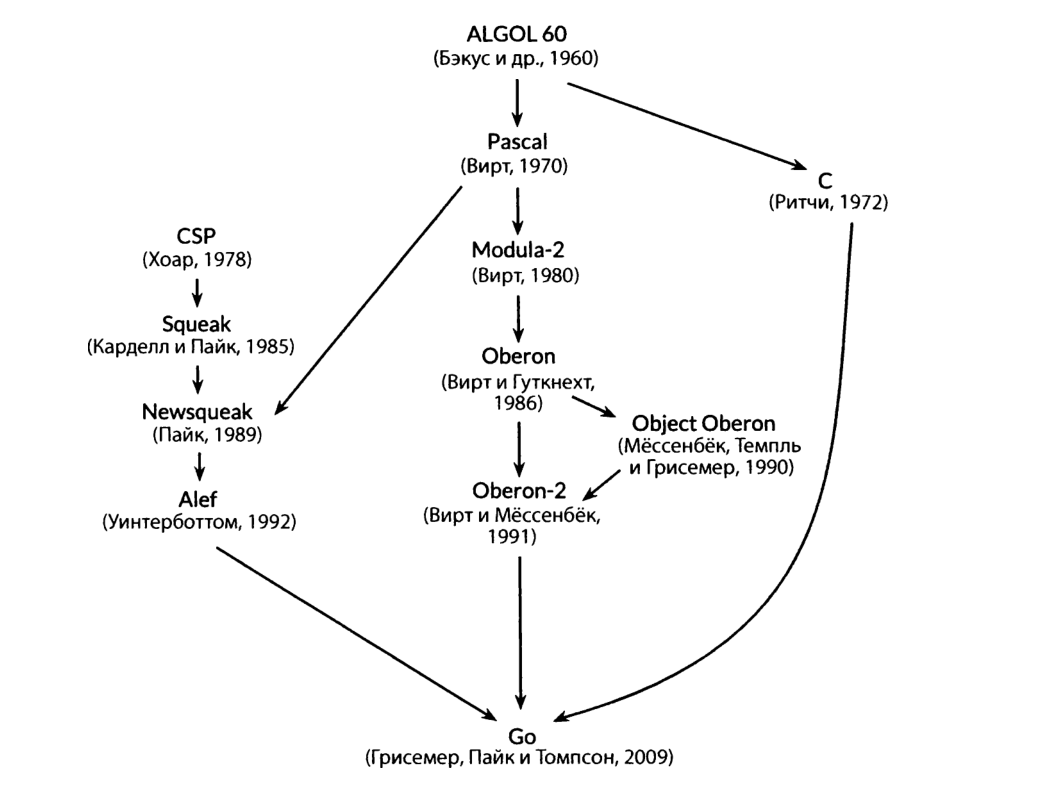
\includegraphics[scale=0.5]{goparents}
		\caption{Родственные связи Go с другими языками}
		\label{goparents}
	\end{figure}
	
	\subsection{Разраобка архитектуры и формата данных}
	Как сказано в \cite{Hoar}: <<Есть два способа конструирования программного обеспечения. Один из них заключается в том, чтобы создавать такие простые программы, в которых нет недостатков; другой --- в том, чтобы создавать программы настолько сложные, чтобы в них не было очевидных недостатков. Первый метод значительно труднее.>>
	
	Следуя принципам проектирования программного обеспечения для операционных систем семейства UNIX, модули тестирования API и само ядро реализующее алгоритм были разработаны раздельно, а для их взаимодействия был разработан текстовый формат обмена данными.
	
	Важныи качеством модульного кода является инкапсуляция. Различные модули не должны зависить от реализации друг друга, а должны взаимодействовать с помощью программных интерфейсов приложений (API) --- набора функций и структур данных, необходимых для работы модулей.
	
	Для взаимодействия модулей тестирования и основного ядра был разработан текстовый протокол взаимодействия так, как текстовые потоки просты для чтения, записи и редактирования человеком без использования специальных средств. Текстовые протоколы являются более масштабируемыми чем бинарные потому, что в двоичных форматах для каждого значения определяется количество выделяемых битов. Данный протокол придерживается DSV-стиля (формат с разделителями значений). В первой строке группы значений записывается количество фигур и шаг поворота, далее идут точки примитивов. Каждая точка записываятся в одну строку, а координаты записаны через пробел. Группы точек между примитивами различных пустой строкой. Признаком конца фигуры, является доветочее, после неё начинается новая фигура. При проектировании формата учитиывались основные соглашения Unix относительно текстовых форматов данных \cite{Unix}.
	
	\subsection{Структуры данных}
	Go является объектно-ориентированным языком программирования и позволяет разграничивать доступ к методам и полям объектов. C++ и подобные языки делают это с помощью модификаторов \lstinline!private! и \lstinline!public!. В языке Go принято использование camel case, и имена приватных полей и методов начинаются с прописной буквы, а публичных --- с заглавной.
	
	
	Рассмотрение структур данных следует начать с представления фигур в системе.
	Для этого используется три структуры. Первая, самая простая --- \lstinline!Point!, которая представляет точку в двумерном пространстве.	Она имеет два открытых поля для: \lstinline!X! и \lstinline!Y! для представления координаты в пространстве.
	\lstinputlisting[caption=Структура представления точки, captionpos=b]{listings/point.go}
	
	Точки объединяются в примитивы с помощью структуры \lstinline|Primitive| имеющей публичное поля типа \lstinline|[]Points| --- срез точек.
	\lstinputlisting[caption=Структура представления примитива, captionpos=b]{listings/primitive.go}
	
	Из примитивов строится фигура, представленная структурой \lstinline|Figure|. Поле \lstinline|ID| необходимо для идентификации фигур, \lstinline|Quant| --- для указания количества повторений данной фигуры при построении множества фигур для раскроя, \lstinline|Matrix| представляет собой матрицу афинного преобразования применённого к данной фигуре в процессе раскроя. Поля\lstinline|Width| и \lstinline|Height| --- ширина и высота фигуры. Поле \lstinline|AngleStep| представляет шаг угла поворота фигуры. \lstinline|[]Primitive| --- срез примитивов, входящих в данную фигуру. \lstinline|MassCenter| --- центр масс данной фигуры.
	\lstinputlisting[caption=Структура представления фигуры, captionpos=b]{listings/figure.go}
	
	Основной структурой для раскроя является \lstinline|Rastr|, которая представляет растровую матрицу фигуры. Она состоит из полей: \lstinline|RastrMatrix| --- целочисленная растровая матрица, \lstinline|Width| и \lstinline|Height| --- ширина и высота матрицы, \lstinline|OuterContour| --- целочисленные координаты точек внешнего контура фигуры в матрице. \lstinline|PointInt| представлена также, как и \lstinline|Point|, но её поля имеют тип \lstinline|int|.
	\lstinputlisting[caption=Структура представления растра, captionpos=b]{listings/rastr.go}
	
	Информация о результате раскроя представляется структурой \lstinline|Position|, состоящей из следующих полей: \lstinline|Fig| --- указатель на фигуру из задания (следует отметитить, что в Go указатели не являются таким мощным типом данных как в Си, в Go отсутствует указательная арифметика, и указатели являются просто ссылками на объект), \lstinline|X| и \lstinline|Y| --- координаты размещения фигуры на плоскости, \lstinline|Angle| --- угол, на который была повёрнута фигура.
	\lstinputlisting[caption=Структура представления результата раскроя, captionpos=b]{listings/position.go}

	
	Основная элемент генетического алгоритма индивид представлен структурой \lstinline|Individual|, состоящей из трёх полей: \lstinline|Height| --- высота раскроя данного индивида, \lstinline|Genom| --- геном или раскройная последовательность, \lstinline|Positions| --- расположение фигур на раскройной плоскости.
	\lstinputlisting[caption=Структура представления индивида генетического алгоритма, captionpos=b]{listings/individual.go}
	
	\subsection{Реализация основных функций и методов}
	Следует упомянуть некоторые идеи и особенности реализации методов и функций в Go. 
	
	Для многих других функций даже в хорошо написанных программах успех не гарантируется, потому что он зависит от факторов, находящихся вне контроля програм­миста. Например, любая функция, выполняющая ввод-вывод, должна  учитывать воз­можность ошибки, и только наивный программист верит в то, что простое чтение или запись никогда не сбоит. Когда наиболее надежные операции неожиданно оказыва­ются неудачными, обязательно необходимо знать, в чем дело.Таким образом, ошибки являются важной частью API пакета или пользовательского интерфейса приложения, и сбой является лишь одним из нескольких ожидаемых поведений программы. В этом 	заключается подход Go к обработке ошибок. Функция, для которой отказ является ожидаемым поведением, возвращает дополнительный результат, обычно последний. Если сбой имеет только одну возможную причину, результат представляет собой булево значение, обычно с именем ok. Чаще всего, и в особенности для ввода-вывода, неудачи могут иметь множество разнообразных причин, так что вызывающая функция должна знать, что именно про­изошло. В таких случаях тип дополнительного результата — error.
	
	В Go нет перегрузки операторов и функций, а методы в Go объявляются с помощью вариации объявления обычных функций, в кото­ром перед именем функции появляется дополнительный параметр. Этот параметр присоединяет функцию к типу этого параметра. Дополнительный параметр называется получателем метода приемника; это на­	звание унаследовано от ранних объектно-ориентированных языков, которые описы­вали вызов метода как “отправку сообщения объекту”. В Go не используется специальное имя, такое как this или self, для получателя; мы выбираем имя для получателя так же, как для любого другого параметра. Поскольку имя получателя будет использоваться часто, лучше выбрать что-то короткое и согласованно используемое во всех методах. В вызове метода аргумент получателя находится перед именем метода \cite{Golang}.

	
	Рассмотрим реализацию функции мутации генетического алгоритма, она является методам типа \lstinline|Individual|. В результате она возвращает кортеж из нового индивида и ошибки, если таковая была. Едиственная аварийная ситуация для данной функции --- слишком маленький геном индивида. Во время выполнения функция копирует геном входного индивида в новый индивид и генерирует два различных случайных числа с индексами массива, затем она меняет местами гены на этих номерах.
	\lstinputlisting[caption=Метод для реализации мутации индивида, captionpos=b]{listings/mutate.go}
	
	Скрещевание индивидов представлено функцией, принимающей на вход указатели на индивидов-родителей. Также как и мутация, она возвращает нового индивида и сообщение об ошибке, если таковая была. Для этой функции возможно две аварийных ситуации: индивиды имели различные длины геномов или же геномы одинаковые, но слишком короткие. После проверки на ошибки, функция генерирует два случайных числа с номерами генов, которые будут взяты из первого родителя и перейдут в ребёнка, далее свободные места заполняются генами второго родителя.
	\lstinputlisting[caption=Функция для реализации скрещевания индивидов, captionpos=b]{listings/crossover.go}
	
	Следующая функция выполняет преобразование растра в фигуру, её первый аргумент  \lstinline|rt| является особенностью данной реализации и не будет рассматриваться. Второй аргумент представляет параметр для масштабирования растра, данное преобразование позволяет за счёт точности увеличить скорость раскроя. Третий аргумент позволяет задать увеличение границы, это необходимо для того, чтобы учесть толщину режущего элемента. В цикле функции выполняется описанный выше алгоритм перехода, для каждого отрезка, входящего в фигуру. Функции заливки, масштабирования и увеличения толщины границ также являются особенностью конкретной реализации и рассматриваться не будут.
	\lstinputlisting[caption=Метод для реализации перехода от фигуры к растру, captionpos=b]{listings/fig_to_rastr.go}
	
	Рассмотрим функцию для раскроя заданной последовательности фигур. Данная функция завершится аварийно если были переданы некорректные параметры: неположительная ширина или высота раскройной плоскости, отрицательная толщина границы или параметр масштабирования. В последовательности фигур могут встречатся фигуры с одинаковым \lstinline|ID|, как только не нашлось места для одной из таких фигур, все следующие пропускаются, такой подход уменьшает время выполнения. Если  на вход пришёл индивид с нулевой длиной --- это значит, что это генерация первичного решения и будут располагаться только фигуры из заданного массива, если же длина генома ненулевая, сначала располагаются фигуры из генома, а затем те из входного массива, которые ещё не были использованы в геноме.
	\lstinputlisting[caption=Функция для раскроя заданной последовательности, captionpos=b]{listings/rastr_nest.go}

	
	Ниже описана функция, для расположения фигуры на плоскости. На вход она принимает указатель на саму фигуру, массив уже расположенных фигур и параметры описанные ранее. Функция работает с копией фигуры и не модифицирует фигуры в пользовательском массиве. В цикле с заданным шагом кгла поворта, выполняется переход от фигуры к растру для фигуры и с шагом в один пиксель происходит проверка расположения фигуры. Расположение фигуры делается сначала на первое подходящее место, затем отыскивыются лучшие места расположения исходя из функции оценки, являющейся особенностью реализации. Если было найдено подходящее расположение фигуры, её растр сохраняется в раскройную плоскость, а вызывающей функции сообщается результат операции.
	\lstinputlisting[caption=Функция расположения фигуры на плоскости, captionpos=b]{listings/place_fig.go}
	
	Рассмотрим основной цикл программы. Выполнение происходит пока во входном наборе есть фигуры. Далее создаётся первоначальное решение, затем в цикле с заданным количеством итераций генетического алгоритма, происходит улучшение базисного решения. Сначала, если есть возможность, происходит операция скрещевания, и для новых индивидов сразу запускается функция раскроя в отдельном потоке. Далее, пока не будет набрано необходимое количество новых индивидов, либо не истечёт число попыток, будет происходить операция мутации. После выполнения цикла генетического алгоритма, на стандартный вывод подаётся информация о расположенных фигурах и отдельный модуль сохраняет результат в файл, далее все расположенные фигуры удаляются из массива и цикл повторяется с генерации базисного решения.
	\lstinputlisting[caption=Цикл основной программы, captionpos=b]{listings/main.go}
	\section{Заключение}
	В процессе исследования было реализовано API на языке программирования Go для разработки систем автоматизированного раскроя. Сравнение алгоритмов и на основе полигонов и растров показало следующие преимущества раскроя с помощью растровых матриц:
	\begin{itemize}
		\item простота реализации;
		\item масштабируемость алгоритма;
		\item более высокая скорость работы при достаточно малой потере точности;
		\item простой поиск свободных мест внутри других фигур.		
	\end{itemize}

	Для наглядности результата, возьмём лист $1063\times1063$ мм. В раскройный план входят следующие наименования фигур:
	\begin{enumerate}
		\item <<Олень>> --- 5 штук, с шагом 15 градусов.
		\item <<Обезьянка>> --- 5 штук, с шагом 15 градусов.
		\item <<Голубь>> --- 5 штук, с шагом 15 градусов.
		\item <<Лошадка>> --- 5 штук, с шагом 15 градусов.
		\item <<Ангелок>> --- 5 штук, с шагом 15 градусов.
	\end{enumerate}


	За $10$ итераций генетического алгоритма были достигнуты следующие результаты:
	\begin{enumerate}
		\item Раскройный план полностью выполнен с использованием двух листов.
		\item Первичная высота раскроя на первом листе --- $298.3$ мм, итоговая высота --- $292.1$ мм.
		\item Первичная высота раскроя на втором листе --- $172.2$ мм, итоговая высота --- $167.4$ мм.
	\end{enumerate}


	Следует отметить, что для примера взят достаточно маленький лист. Экономия материала линейно возрастает с увеличением площади. Результаты можно увидеть на рис. \ref{plane12}.
	\begin{figure}[h]
		\centering
		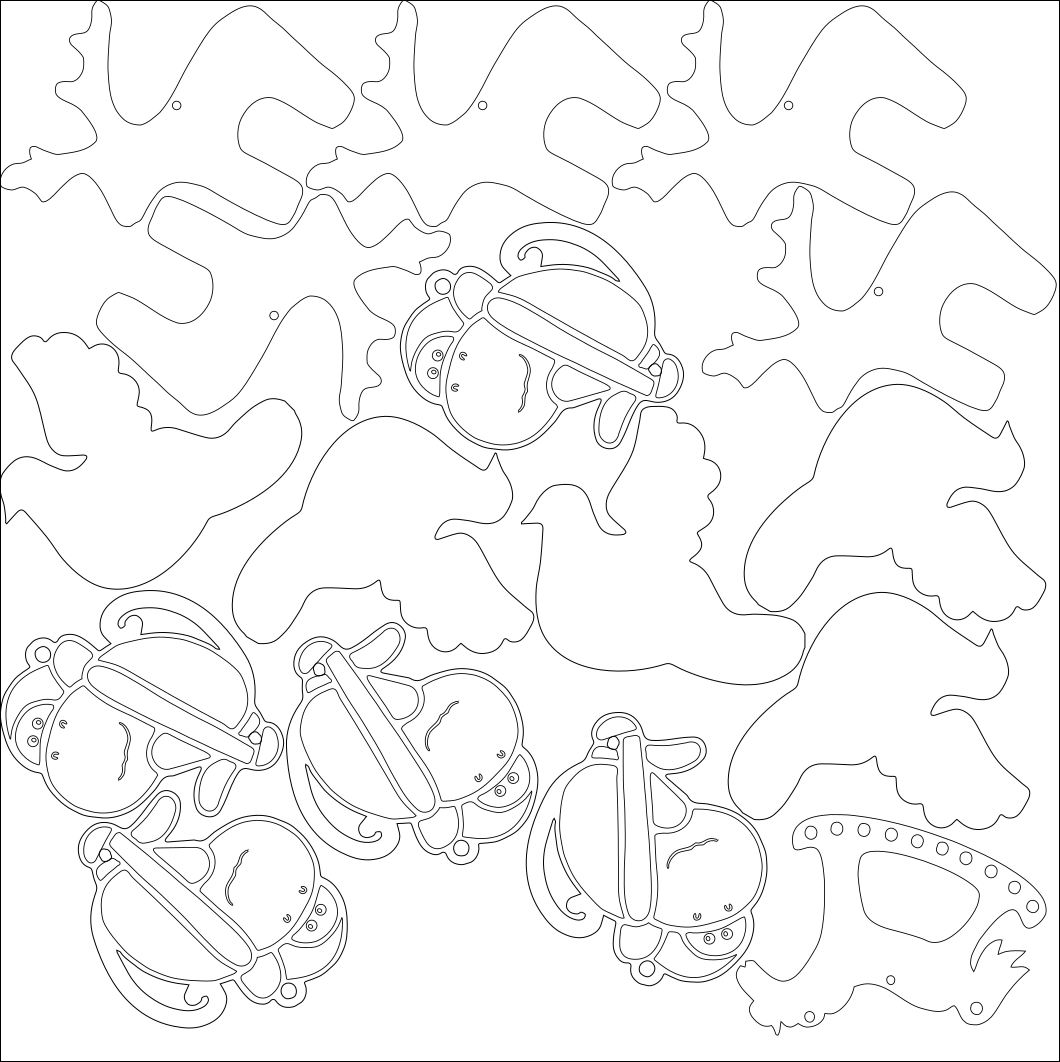
\includegraphics[scale=0.18]{plane1}
		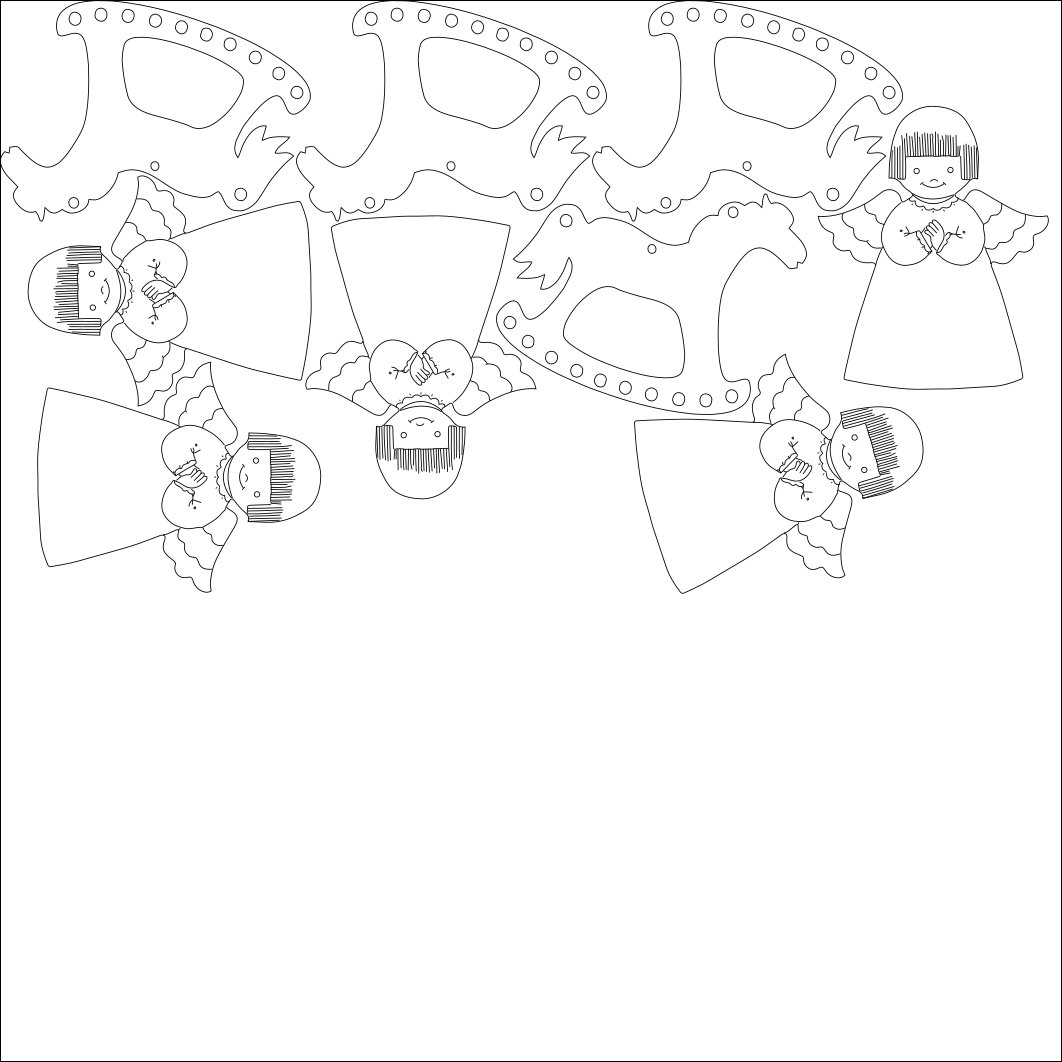
\includegraphics[scale=0.18]{plane2}
		\caption{Первый и второй раскройные листы}
		\label{plane12}
	\end{figure}
	\begin{thebibliography}{1}
		\bibitem{Dyckhoff} Dyckhoff H. A typology of cutting and packing problems // European Journal of Operational Research. № 44. 150---152 p.
		\bibitem{Cantorovich} Залгаллер В. А., Канторович Л. В. Рациональный раскрой промышленных материалов. Новосибирск: Наука, 1971.
		\bibitem{Nikitenkov} Никитенков В. Л., Холопов А. А. Задачи линейного программирования и методы их решения. Сыктывкар: Издательство Сыктывкарского университета, 2008. 143 с.
		\bibitem{Parsolov}  Прасолов В. В. Задачи по планиметрии. --- 4-е изд., дополненное. М.: МЦНМО, 2001. 584 с 
		\bibitem{Shabat} Шабат Б. В. Введение в комплексный анализ. М.: Наука, 1969. 91 с.
		\bibitem{Benell_Olivera} Benell A. J., Olivera F. J. The geometry of nesting problems: A tutorial // European Journal of Operational Research. 2008. № 184. 399---402 p.
		\bibitem{McLeod} MacLeod C. An Introduction to Practical Neural Networks and Genetic Algorithms For Engineers and Scientists. 85 p.
		\bibitem{China} He Y., Liu H. Algorithm for 2D irregular-shaped nesting problem based on the NFP algorithm and lowest gravity-center principle // Journal of Zhejiang University. 2006. № 7. 571 --- 574 p.
		\bibitem{GA} Панченко Т. В. Генетические Алгоритмы; под ред. Ю. Ю. Тарасевича. Издательский дом <<Астраханский университет>>. 2007. 16 с.
		\bibitem{Kudryavcev} Кудрявцев Л. Д. Математический анализ. --- 2-е изд.  М.: Высшая школа, 1973. --- Т. 1.
		\bibitem{Golang} Донаван А. А. А., Керниган Б. У. Язык программировния Go. М., СПб., Киев: Вильямс, 2016. 11---12 с., 160---161 с., 191---192 с.
		\bibitem{Hoar} Хоар Ч. А. Р. The Emperor’s Old Clothes. CACM, 1981.
		\bibitem{Unix} Реймонд Э. С. Искусство программирования для UNIX. CACM, М., СПб., Киев: Вильямс, 2005.
	\end{thebibliography}
\end{document}